% !TeX program = xelatex
% Overleaf: choose XeLaTeX and main.tex. All required figures are included.
% The magic comment above does not change the compiler in Overleaf settings.
\RequirePackage{iftex}
\RequireXeTeX
\documentclass[aspectratio=169,11pt]{beamer}
\usepackage[UTF8,scheme=plain,fontset=fandol]{ctex}
\usepackage{amsmath,amssymb,booktabs,graphicx,tikz}
\usetikzlibrary{arrows.meta,positioning,calc}
% The Overleaf ZIP places all five PNGs beside main.tex.
% The repository keeps them in figures/; both layouts are supported.
\graphicspath{{./}{figures/}}

\definecolor{Navy}{HTML}{192E49}
\definecolor{Teal}{HTML}{167E89}
\definecolor{Amber}{HTML}{C87921}
\definecolor{Muted}{HTML}{607087}
\definecolor{Pale}{HTML}{EDF5F7}
\setbeamercolor{normal text}{fg=Navy,bg=white}
\setbeamercolor{structure}{fg=Teal}
\setbeamercolor{frametitle}{fg=Navy,bg=white}
\setbeamercolor{block title}{fg=Teal,bg=Pale}
\setbeamercolor{block body}{fg=Navy,bg=Pale}
\setbeamercolor{takeaway}{fg=Navy,bg=Pale}
\setbeamercolor{alerted text}{fg=Amber}
\setbeamerfont{frametitle}{size=\Large,series=\bfseries}
\setbeamerfont{block title}{size=\normalsize,series=\bfseries}
\setbeamertemplate{navigation symbols}{}
\setbeamertemplate{itemize item}{\small\raisebox{0.15ex}{\textbullet}}
\setbeamertemplate{itemize subitem}{\scriptsize\textbullet}
\setbeamersize{text margin left=0.8cm,text margin right=0.8cm}
\setbeamertemplate{frametitle}{%
  \vspace{0.08cm}\insertframetitle\par\vspace{0.08cm}%
  {\color{Teal}\rule{\linewidth}{0.7pt}}\vspace{-0.08cm}}
\newcommand{\deckpage}{\insertframenumber\,/\,13}
\setbeamertemplate{footline}{%
  \leavevmode\hbox{%
  \begin{beamercolorbox}[wd=.86\paperwidth,ht=0.34cm,dp=0.16cm,leftskip=.8cm]{normal text}
    \color{Muted}\fontsize{7}{9}\selectfont
    Calzona, Bauer \& Trauzettel \enspace|\enspace SciPost Phys. Core 3, 014 (2020)
  \end{beamercolorbox}%
  \begin{beamercolorbox}[wd=.14\paperwidth,ht=0.34cm,dp=0.16cm,rightskip=.8cm plus1fil]{normal text}
    \hfill\color{Muted}\footnotesize\deckpage
  \end{beamercolorbox}}}
\newcommand{\source}[1]{{\par\vspace{0.1cm}\fontsize{7.5}{10}\selectfont\color{Muted}#1\par}}
\newcommand{\takeaway}[1]{%
  \begin{beamercolorbox}[wd=\linewidth,sep=0.6em]{takeaway}\small #1\end{beamercolorbox}}
\newcommand{\ket}[1]{\lvert #1\rangle}
\newcommand{\bra}[1]{\langle #1\rvert}
\newcommand{\iu}{\mathrm{i}}
\newcommand{\Uent}{U_{\mathrm{ent}}}
\newcommand{\Hhad}{H_{\mathrm{Had}}}
\DeclareMathOperator{\diag}{diag}
\hypersetup{colorlinks=true,urlcolor=Teal,
  pdftitle={Majorana 量子比特 CNOT 门的几何实现},
  pdfsubject={文献汇报：arXiv:2008.05181}}

\begin{document}

% 1 -------------------------------------------------------------------
\begin{frame}[plain,shrink=2]
  \vspace{0.6cm}
  {\color{Teal}\large 文献汇报}\par\vspace{0.4cm}
  {\huge\bfseries Majorana 量子比特\\[0.22cm]CNOT 门的几何实现}\par
  \vspace{0.4cm}
  {\color{Teal}\rule{2.2cm}{2pt}}\par\vspace{0.35cm}
  {\large Holonomic implementation of CNOT gate\\[0.08cm]
  on topological Majorana qubits}\par\vspace{0.4cm}
  A. Calzona, N. P. Bauer, B. Trauzettel\par\vspace{0.15cm}
  {\color{Muted}SciPost Physics Core \textbf{3}, 014 (2020)}\par
  \vspace{0.55cm}
  \takeaway{条件耦合 $\longrightarrow$ 几何相位 $\longrightarrow$ 两比特纠缠门}
  \source{理论方案与数值模拟\quad
  \href{https://doi.org/10.21468/SciPostPhysCore.3.2.014}{doi:10.21468/SciPostPhysCore.3.2.014}
  \quad arXiv:2008.05181}
\end{frame}

% 2 -------------------------------------------------------------------
\begin{frame}[t,shrink=2]{背景与创新：从单比特编织走向两比特纠缠}
  \begin{columns}[T,onlytextwidth]
    \begin{column}{0.48\textwidth}
      \begin{block}{研究动机}
        \begin{itemize}\setlength{\itemsep}{0.16cm}
          \item 单比特内部编织可以实现一部分逻辑门。
          \item 两比特操作还需要产生\textbf{纠缠}。
          \item 在各自固定宇称的编码下，直接跨比特交换可能离开计算空间。
        \end{itemize}
      \end{block}
    \end{column}
    \begin{column}{0.48\textwidth}
      \begin{block}{本文的推进}
        \begin{itemize}\setlength{\itemsep}{0.16cm}
          \item 用\textbf{闭环绝热控制}产生条件几何相位。
          \item 提出四模相互作用与双隧穿两种协议。
          \item 检查有限操作时间、寄生耦合及通道不对称的影响。
        \end{itemize}
      \end{block}
    \end{column}
  \end{columns}
  \vspace{0.12cm}
  \small
  \textbf{已有基础：}耦合控制的编织 [31]；可调相互作用与投影操作的联系 [34]；
  Majorana 浮置岛架构 [35]。
  \vspace{0.12cm}
  \takeaway{本文具体构造了两比特几何门；门执行过程中无需联合宇称投影测量。}
  \source{参考文献编号沿用原论文；完整条目见备用页。}
\end{frame}

% 3 -------------------------------------------------------------------
\begin{frame}[t]{模型：四个 Majorana 编码，两个提供辅助耦合}
  \begin{columns}[T,onlytextwidth]
    \begin{column}{0.42\textwidth}
      每个量子比特包含六个模式：
      \begin{itemize}\setlength{\itemsep}{0.12cm}
        \item 编码：$\gamma_1,\gamma_2,\gamma_3,\gamma_4$；
        \item 辅助：$\gamma_0,\gamma_5$。
      \end{itemize}
      \[
        P_{jk}=\iu\gamma_j\gamma_k=1-2n_{jk}.
      \]
      固定总偶宇称，空闲时选取
      \[
      \begin{aligned}
        \ket{0}_{\mathrm L}&=\ket{0,0,0},\\
        \ket{1}_{\mathrm L}&=\ket{1,1,0}.
      \end{aligned}
      \]
      \small 占据数顺序：$(n_{12},n_{34},n_{05})$。\\
      两个逻辑态都处于低能空间。
    \end{column}
    \begin{column}{0.55\textwidth}
      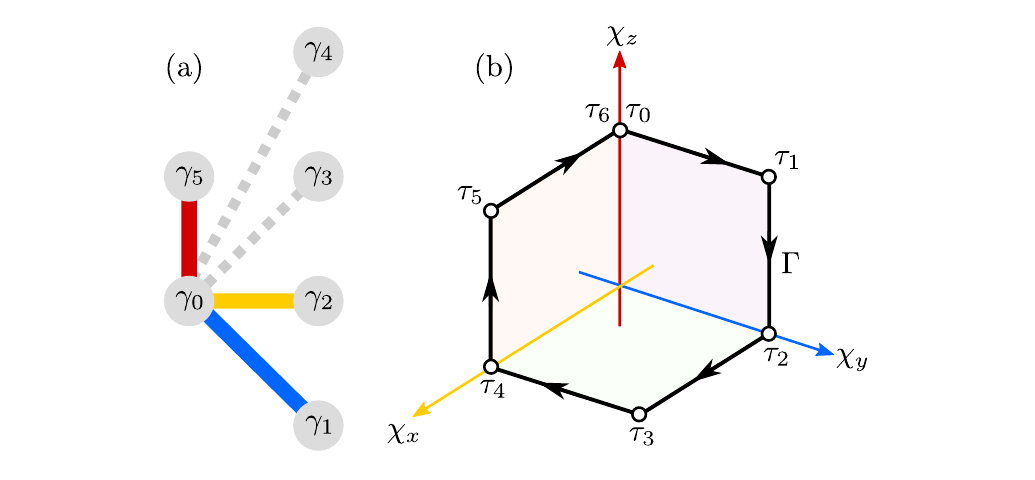
\includegraphics[width=\linewidth]{paper_fig1.png}
      \source{原文 Fig. 1：模式连接与耦合参数闭环。}
      \vspace{0.18cm}
      \small
      \[
        H=-\chi_xP_{02}-\chi_yP_{01}-\chi_zP_{05}.
      \]
      空闲设置：$\chi_z=\Theta>0$，$\chi_x=\chi_y=0$。\\[0.1cm]
      辅助对被锁定在 $P_{05}=+1$。
    \end{column}
  \end{columns}
\end{frame}

% 4 -------------------------------------------------------------------
\begin{frame}[t,shrink=2]{几何门：参数回到起点，量子态留下相位}
  \small
  控制三个耦合，按六段路径完成一个闭环：
  \vspace{0.2cm}
  {\centering
    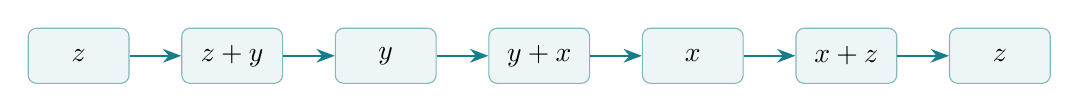
\begin{tikzpicture}[>=Stealth,
      state/.style={draw=Teal!55,fill=Pale,rounded corners=3pt,
        minimum width=1.28cm,minimum height=.7cm,font=\normalsize}]
      \foreach \label [count=\j from 0] in {$z$,$z+y$,$y$,$y+x$,$x$,$x+z$,$z$}{
        \node[state] (s\j) at ({1.95*\j},0) {\label};
      }
      \foreach \j in {0,...,5}{
        \pgfmathtruncatemacro{\k}{\j+1}
        \draw[->,thick,Teal] (s\j)--(s\k);
      }
    \end{tikzpicture}
  \par}
  \begin{columns}[T,onlytextwidth]
    \begin{column}{0.47\textwidth}
      \begin{block}{绝热跟随}
        新耦合开启后，再关闭旧耦合。\\[0.12cm]
        保持能隙，缓慢改变控制参数，使状态跟随瞬时基态。
        \[
          \Delta=2\sqrt{\chi_x^2+\chi_y^2+\chi_z^2}>0.
        \]
      \end{block}
    \end{column}
    \begin{column}{0.49\textwidth}
      \begin{block}{相对相位来自几何}
        \[
          \ket{g(0)}\ \longrightarrow\
          e^{\iu\phi_{\rm dyn}}e^{\iu\phi_{\rm geo}}\ket{g(0)}.
        \]
        简并分支的动力学相位相同。\\[0.12cm]
        几何相位取决于参数路径；二能级问题中与立体角的一半相关。
      \end{block}
    \end{column}
  \end{columns}
  \vspace{0.15cm}
  \takeaway{归一化参数方向沿 $z\to y\to x\to z$ 走过球面八分之一，立体角大小为 $\pi/2$。}
  \source{此页能隙为单比特／四模协议的二能级块结果；双隧穿模型须单独检查能隙。}
\end{frame}

% 5 -------------------------------------------------------------------
\begin{frame}[t,shrink=2]{方案一：四 Majorana 耦合产生条件几何相位}
  \[
    H^{4\gamma}=-\chi_xP_{02}^{B}
       -{\color{Teal}\chi_yP_{12}^{A}P_{01}^{B}}
       -\chi_zP_{05}^{B}.
  \]
  \begin{columns}[T,onlytextwidth]
    \begin{column}{0.47\textwidth}
      \small
      \textbf{控制比特 $A$ 决定耦合符号}
      \[
        P_{12}^{A}=\begin{cases}
          +1,&A=0,\\
          -1,&A=1.
        \end{cases}
      \]
      一条有效耦合反号，改变几何相位。\\[0.18cm]
      四模项在每个比特中包含两个 Majorana，保持各自总宇称。
    \end{column}
    \begin{column}{0.49\textwidth}
      \small
      \textbf{四个逻辑分支获得不同相位}
      \[
        \phi_{nm}=(-1)^{n+m}\frac{\pi}{4}.
      \]
      \centering
      \begin{tabular}{cc}
        \toprule
        逻辑态 & 几何相位\\
        \midrule
        $\ket{00},\ket{11}$ & $+\pi/4$\\
        $\ket{01},\ket{10}$ & $-\pi/4$\\
        \bottomrule
      \end{tabular}
    \end{column}
  \end{columns}
  \vspace{0.1cm}
  \takeaway{闭环得到 $U_{\rm geo}=e^{\iu\pi Z_AZ_B/4}$；去掉整体相位后，
  $\Uent=\diag(1,-\iu,-\iu,1)$。}
  \source{$Z_A,Z_B$ 为逻辑 Pauli 算符；上述门由含辅助模式的完整闭环产生。}
\end{frame}

% 6 -------------------------------------------------------------------
\begin{frame}[t,shrink=2]{从几何纠缠门构造 CNOT}
  \small
  单比特相位修正先将 $\Uent$ 转为受控相位门：
  \[
    S=\diag(1,\iu),\qquad
    (S\otimes S)\Uent=\diag(1,1,1,-1)=CZ.
  \]
  再对目标比特做基变换，利用 $\Hhad Z\Hhad=X$：
  \[
    \boxed{CNOT_{A\to B}
      =(I\otimes\Hhad)(S\otimes S)\Uent(I\otimes\Hhad).}
  \]
  {\centering
  \begin{tikzpicture}[>=Stealth,
    gate/.style={draw=Teal,fill=white,minimum width=.7cm,minimum height=.6cm},
    font=\small]
    \draw[thick] (0,1.1)--(11.8,1.1);
    \draw[thick] (0,0)--(11.8,0);
    \node[left] at (0,1.1) {$A$};
    \node[left] at (0,0) {$B$};
    \node[gate] at (1.5,0) {$\Hhad$};
    \filldraw[fill=Pale,draw=Teal,thick,rounded corners=3pt]
       (3.2,-.35) rectangle (5.7,1.45);
    \node at (4.45,.55) {$\Uent$};
    \node[Teal] at (4.45,1.78) {几何闭环};
    \node[gate] at (7.3,1.1) {$S$};
    \node[gate] at (7.3,0) {$S$};
    \node[gate] at (9.5,0) {$\Hhad$};
    \draw[->,Muted] (1,-.8)--(10.6,-.8)
      node[midway,below,font=\scriptsize] {实际执行顺序：从左到右};
  \end{tikzpicture}
  \par}
  \takeaway{$\ket{a,b}\mapsto\ket{a,b\oplus a}$：$A=0$ 时保持目标比特，$A=1$ 时翻转目标比特。}
\end{frame}

% 7 -------------------------------------------------------------------
\begin{frame}[t,shrink=2]{方案二：用两条跨岛隧穿通道实现条件耦合}
  \begin{columns}[T,onlytextwidth]
    \begin{column}{0.35\textwidth}
      \small
      \textbf{两条普通隧穿通道}
      \[
      \begin{aligned}
        I_{20}&=\iu\gamma_2^A\gamma_0^B,\\
        I_{11}&=\iu\gamma_1^A\gamma_1^B.
      \end{aligned}
      \]
      \textbf{加上充电项}
      \[
        H_E=-E(P^A+P^B),\quad E>0.
      \]
      $P^A,P^B$ 表示各岛的总宇称。\\[0.1cm]
      两条通道在部分时间内\textbf{共同开启}。
    \end{column}
    \begin{column}{0.62\textwidth}
      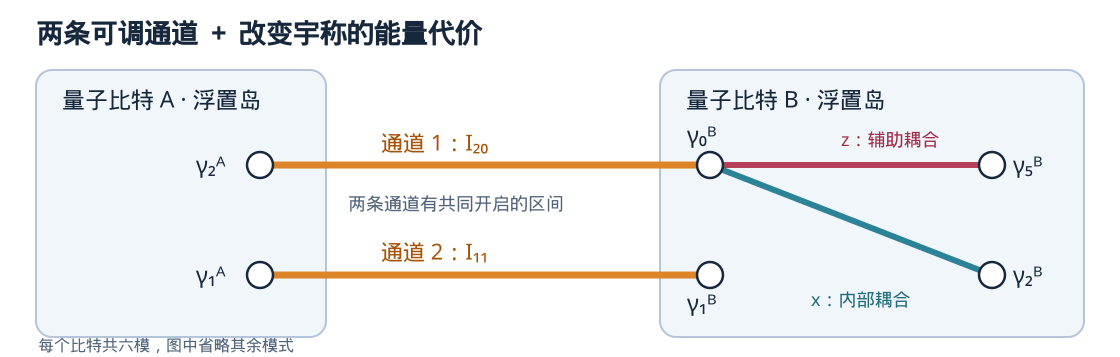
\includegraphics[width=\linewidth]{double_tunneling_channels.png}
      \source{根据论文模型绘制；每个比特六个模式，图中省略其余模式。}
    \end{column}
  \end{columns}
  \vspace{0.08cm}
  \[
    H^{\rm dt}=H_E-\chi_xP_{02}^{B}
       -\chi_y(I_{20}+I_{11})-\chi_zP_{05}^{B}.
  \]
  \takeaway{两条跨岛通道、岛内耦合及辅助耦合共同完成闭环，产生两比特几何门。}
\end{frame}

% 8 -------------------------------------------------------------------
\begin{frame}[t]{充电能的作用：抑制单次隧穿，保留二阶协同作用}
  \small
  单次隧穿本身就会翻转两个岛的宇称；充电能为这种变化设置能量代价。
  \begin{center}
  \begin{tikzpicture}[>=Stealth,font=\small,
    sector/.style={draw=Teal!40,fill=Pale,rounded corners=3pt,
      minimum width=2.7cm,minimum height=1cm,align=center}]
    \node[sector] (a) at (0,0) {偶--偶\\充电项能量 $-2E$};
    \node[sector,fill=Amber!12,draw=Amber!50] (b) at (4.7,0)
      {奇--奇\\充电项能量 $+2E$};
    \node[sector] (c) at (9.4,0) {偶--偶\\恢复原宇称扇区};
    \draw[->,thick] (a)--node[above,font=\scriptsize] {一条通道} (b);
    \draw[->,thick] (b)--node[above,font=\scriptsize] {另一条通道} (c);
    \node[below=.15cm of b,Amber] {中间态多付出 $4E$};
  \end{tikzpicture}
  \end{center}
  \vspace{-0.12cm}
  大 $E$ 下，两种先后次序的\textbf{虚过程}共同给出
  \[
  \begin{aligned}
    I_{20}I_{11}&=P_{12}^{A}P_{01}^{B},\\[-0.04cm]
    H_{\rm eff}^{(2)}
      &=-\frac{\chi_y^2}{4E}(I_{20}+I_{11})^2
       =-\frac{\chi_y^2}{2E}I
        -\frac{\chi_y^2}{2E}P_{12}^{A}P_{01}^{B}.
  \end{aligned}
  \]
  \takeaway{第二项正是方案一的四模耦合；第一项只带来共同能量修正。}
  \source{这是大充电能下的二阶解释，箭头不表示两个依次执行的真实跳跃。
  论文还用完整模型证明：有限正 $E$ 下，指定绝热闭环得到同一门；过程中可含奇--奇成分。}
\end{frame}

% 9 -------------------------------------------------------------------
\begin{frame}[t]{Fig. 3(b)：四重简并的基态与有限能隙}
  \begin{columns}[T,onlytextwidth]
    \begin{column}{0.51\textwidth}
      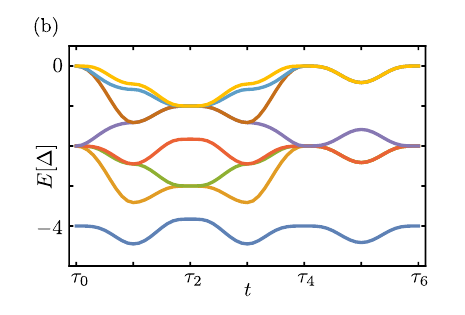
\includegraphics[width=\linewidth,height=4.5cm,keepaspectratio]{paper_fig3b.png}
      \source{原文 Fig. 3(b)，仅显示负能量部分。\\
      横轴：六段控制过程；纵轴：瞬时能量。}
    \end{column}
    \begin{column}{0.46\textwidth}
      \small
      \textbf{最低蓝线：四个基态重合}\\[0.12cm]
      四个逻辑分支保持简并，动力学相位相同。\\[0.25cm]
      \textbf{与激发态始终分离}\\[0.12cm]
      最低线到最近激发能级的间隔 $\Delta(t)>0$，支持绝热跟随。\\[0.25cm]
      \textbf{上方交叉不关闭基态能隙}\\[0.12cm]
      其他曲线是激发能级；负能量也可以对应激发态。
    \end{column}
  \end{columns}
  \vspace{0.25cm}
  \takeaway{能谱说明“可以留在简并基态空间”；具体实现哪个门，还需计算几何相位。}
\end{frame}

% 10 ------------------------------------------------------------------
\begin{frame}[t,shrink=2]{控制与验证：如何判断协议实现了目标门}
  \begin{columns}[T,onlytextwidth]
    \begin{column}{0.47\textwidth}
      \begin{block}{控制方法}
        \small
        沿六段闭环开关耦合，每段时长 $T/6$。采用平滑余弦插值
        \[
          g(s)=\frac{1-\cos(\pi s)}{2},\quad 0\le s\le1.
        \]
        $s$ 是该段的归一化时间，$T$ 为总操作时间。
      \end{block}
    \end{column}
    \begin{column}{0.49\textwidth}
      \begin{block}{解析与数值方法}
        \small
        \begin{enumerate}\setlength{\itemsep}{0.1cm}
          \item 瞬时能谱：检查基态简并与能隙。
          \item 几何相位：确定闭环对应的门矩阵。
          \item QuTiP 演化：计算有限时间的输出误差。
        \end{enumerate}
      \end{block}
    \end{column}
  \end{columns}
  \vspace{0.1cm}
  \small
  数值输入为 $\ket{++}$，理想输出为 $\ket{\psi_{\rm ent}}=\Uent\ket{++}$：
  \[
    F_\psi(T)=\left|\bra{\psi_{\rm ent}}\psi(T)\rangle\right|^2.
  \]
  \takeaway{本文展示有效模型的理论与数值结果；$F_\psi$ 是指定输入的态保真度。}
\end{frame}

% 11 ------------------------------------------------------------------
\begin{frame}[t]{主要结果：慢操作提高保真度，充电能存在折中}
  \begin{center}
    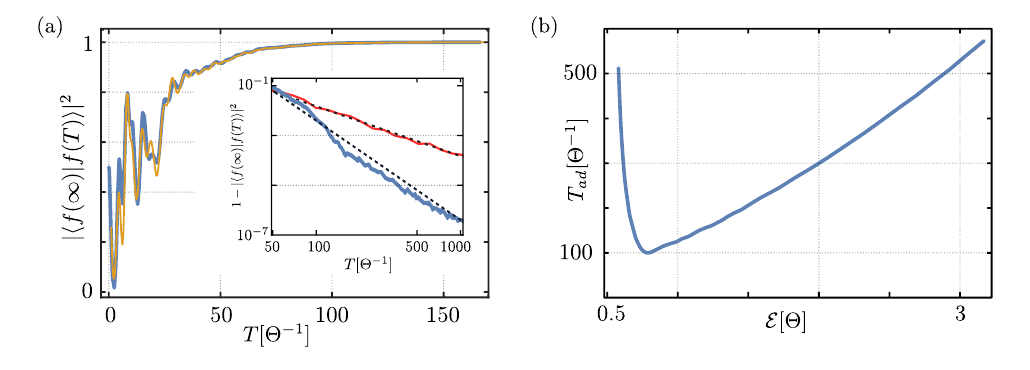
\includegraphics[width=.90\linewidth,height=3.5cm,keepaspectratio]{paper_fig4.png}
  \end{center}
  \vspace{-0.1cm}
  \begin{columns}[T,onlytextwidth]
    \begin{column}{0.31\textwidth}
      \small\textbf{左图：有限时间演化}\\[0.12cm]
      快操作产生非绝热跃迁与干涉振荡；随 $T$ 增大，$F_\psi\to1$。
    \end{column}
    \begin{column}{0.31\textwidth}
      \small\textbf{插图：脉冲平滑性}\\[0.12cm]
      余弦开关：$1-F_\psi\sim T^{-4}$。\\[0.08cm]
      线性开关：$1-F_\psi\sim T^{-2}$。
    \end{column}
    \begin{column}{0.32\textwidth}
      \small\textbf{右图：充电能的折中}\\[0.12cm]
      $E$ 太小，能隙变小；$E$ 太大，有效耦合 $\chi_y^2/(2E)$ 变弱。
    \end{column}
  \end{columns}
  \source{原文 Fig. 4。橙线包含指定寄生耦合；$T_{\rm ad}$ 定义为其后所有操作时长均满足误差 $<10^{-3}$ 的阈值。
  图中采用 $\hbar=1$ 的时间单位。}
\end{frame}

% 12 ------------------------------------------------------------------
\begin{frame}[t]{附录 A、B：解析依据与通道不对称检验}
  \begin{columns}[T,onlytextwidth]
    \begin{column}{0.48\textwidth}
      \begin{block}{附录 A：几何相位怎样得到？}
      \small
      利用守恒宇称分块，再求基态与 Berry 曲率。\\[0.18cm]
      四模协议：相关块为 $2\times2$。\\[0.1cm]
      双隧穿协议：相关块为 $4\times4$。\\[0.18cm]
      虽然曲率形状不同，指定闭环的积分给出相同的
      \[
        \Uent=\diag(1,-\iu,-\iu,1).
      \]
      这提供有限 $E$ 下的解析依据。
      \end{block}
    \end{column}
    \begin{column}{0.48\textwidth}
      \begin{block}{附录 B：通道不相同是否可行？}
      \small
      独立调节 $\chi_{y_1}(t),\chi_{y_2}(t)$，采用八段路径。
      \end{block}
      \begin{center}
        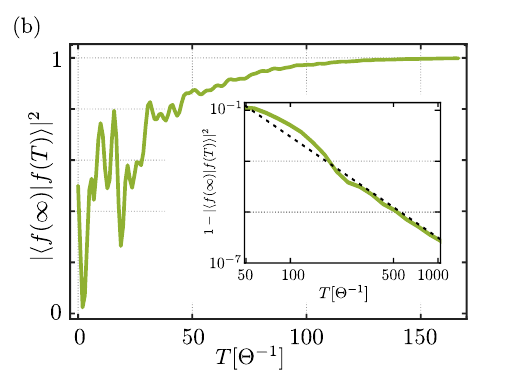
\includegraphics[height=2.35cm,width=\linewidth,keepaspectratio]{paper_fig6b.png}
      \end{center}
      \vspace{-0.1cm}
      \small
      峰值取 $1.2\Theta$、$0.8\Theta$：足够慢时仍得到目标门。
    \end{column}
  \end{columns}
  \source{右图：原文 Fig. 6(b)。两条通道不必严格匹配，但需按协议配合开启，保护不覆盖任意噪声。}
\end{frame}

% 13 ------------------------------------------------------------------
\begin{frame}[t]{本文贡献与适用边界}
  \vspace{0.15cm}
  \begin{block}{门的构造}
    四 Majorana 条件耦合 $\longrightarrow$ 闭环几何相位
    $\longrightarrow$ 纠缠门 $\Uent$\\[0.1cm]
    配合单比特 $S$ 与 Hadamard 门，即可得到 CNOT。
  \end{block}
  \vspace{0.12cm}
  \begin{block}{实现机制}
    两条跨岛隧穿通道加充电能，可产生所需的有效四模作用；
    完整有限 $E$ 模型支持同一绝热几何门。
  \end{block}
  \vspace{0.12cm}
  \begin{block}{数值证据与限制}
    平滑脉冲、合适的充电能与足够慢的控制，有助于降低误差。\\[0.1cm]
    已检验特定寄生耦合及通道不对称；实际器件实现仍待验证。
  \end{block}
\end{frame}

\appendix
\renewcommand{\deckpage}{备用页}

% Backup A -------------------------------------------------------------
\begin{frame}[t]{备用：什么是“有效二能级基态”？}
  \small
  固定一个逻辑分支后，相关状态构成二维空间。
  例如 $B$ 的逻辑 $0$ 分支，按 $(n_{12},n_{34},n_{05})$ 记占据数：
  \[
    \underbrace{\ket{0,0,0}}_{\text{空闲时能量 }-\Theta}
    \qquad\longleftrightarrow\qquad
    \underbrace{\ket{1,0,1}}_{\text{空闲时能量 }+\Theta}.
  \]
  \begin{itemize}\setlength{\itemsep}{0.16cm}
    \item 耦合开启后，瞬时基态是叠加态：
      $\ket{g(t)}=a(t)\ket{0,0,0}+b(t)\ket{1,0,1}$。
    \item 每个二能级块的本征能量为
      $E_\pm=\pm\sqrt{\chi_x^2+\chi_y^2+\chi_z^2}$；基态对应 $E_-$。
    \item 四个逻辑分支各有一个基态，组成四维简并基态子空间。
  \end{itemize}
  \vspace{0.2cm}
  \takeaway{逻辑 $\ket{0}$ 与 $\ket{1}$ 都属于计算用的基态空间；
  “二能级”描述各分支内部的基态与激发态。}
  \source{此解释针对单比特／四模协议；有限充电能的双隧穿模型有额外宇称自由度，相关块为四维。}
\end{frame}

% Backup B -------------------------------------------------------------
\begin{frame}[t,shrink=2]{备用：论文与相关工作}
  \small
  \textbf{本文}\\[0.1cm]
  A. Calzona, N. P. Bauer, B. Trauzettel,\\
  \emph{Holonomic implementation of CNOT gate on topological Majorana qubits}.\\
  SciPost Phys. Core \textbf{3}, 014 (2020).\\
  \href{https://doi.org/10.21468/SciPostPhysCore.3.2.014}{doi:10.21468/SciPostPhysCore.3.2.014}
  \vspace{0.35cm}
  \begin{description}\setlength{\itemsep}{0.18cm}
    \item[{[31]}] B. van Heck et al.,
      \emph{Coulomb-assisted braiding of Majorana fermions in a Josephson junction array}.
      New J. Phys. \textbf{14}, 035019 (2012).
    \item[{[34]}] P. Bonderson,
      \emph{Measurement-only topological quantum computation via tunable interactions}.
      Phys. Rev. B \textbf{87}, 035113 (2013).
    \item[{[35]}] T. Karzig et al.,
      \emph{Scalable designs for quasiparticle-poisoning-protected topological quantum computation with Majorana zero modes}.
      Phys. Rev. B \textbf{95}, 235305 (2017).
  \end{description}
  \source{图像来源：论文 Fig. 1、3(b)、4、6(b)；双隧穿结构图根据论文模型重新绘制。}
\end{frame}

\end{document}
